%%==================================================
%% diss.tex for SJTU Course Design Thesis
%% based on CASthesis, SJTU master thesis
%% modified by icetiny@gmail.com
%% version: 0.3a
%% Encoding: UTF-8
%% last update: Dec 5th, 2010
%%==================================================

% 字号选项: c5size 五号(默认)
% 字号选项: cs4size 小四
% 双面打印(注意字号设置)
%\documentclass[cs4size, a4paper, cs4size, twoside]{sjtumaster-xetex} 
% 单面打印(注意字号设置)
\documentclass[cs4size, a4paer, cs4size, oneside, openany]{sjtumaster-xetex} 
\usepackage{xeCJK}
%\usepackage{multirow}
% \usepackage[sectionbib]{chapterbib}%每章都用参考文献

%\newboolean{DOIT}
%\setboolean{DOIT}{false}%编译某些只想自己看的内容,编译true,否则false

%% 行距缩放因子(x倍字号)
\renewcommand{\baselinestretch}{1.3}

% 设置图形文件的搜索路径
\graphicspath{{figure/}{figures/}{logo/}{logos/}{graph/}{graphs}}

%%========================================
%% 在sjtumaster-xetex.cls中定义的有用命令
%%========================================
% \cndash 中文破折号
% 数学常量
% \me 对数常数e
% \mi 虚数单位i
% \mj 虚数单位j
% \dif 直立的微分算符d为直立体。
% 可伸长的数学箭头、等号
% \myRightarrow{}{}
% \myLeftarrow{}{}
% \myBioarrow{}{}
% \myLongEqual{}{}
% 参考文献
% \upcite{} 上标引用
%%========================================


\begin{document}

%%%%%%%%%%%%%%%%%%%%%%%%%%%%%% 
%% 封面
%%%%%%%%%%%%%%%%%%%%%%%%%%%%%% 

% 中文封面内容(关注内容而不是形式)
\title{交通信号灯控制系统}
\author{孙\quad{}楠}
\advisor{张银桥}
\degree{本科}
\defenddate{2011年6月18日}
\school{上海交通大学}
\institute{机械与动力工程学院}
\studentnumber{5080209271}
\major{机械工程与自动化}

% 英文封面内容(关注内容而不是表现形式)
\englishtitle{\XeTeX/\LaTeX\, Template for SJTU Mater Degree Thesis \version}
\englishauthor{\textsc{Si Li}}
\englishadvisor{Prof. \textsc{San Zhang}}
\englishschool{Shanghai Jiao Tong University}
\englishinstitute{\textsc{Depart of XXX, School of XXX} \\
  \textsc{Shanghai Jiao Tong University} \\
  \textsc{Shanghai, P.R.China}}
\englishdegree{Master}
\englishmajor{Physics}
\englishdate{Jan. 16th, 2010}

% 封面
\maketitle

% 英文封面
%\makeenglishtitle

% 论文原创性声明和使用授权
%\makeDeclareOriginal
%\makeDeclareAuthorization

%%%%%%%%%%%%%%%%%%%%%%%%%%%%%% 
%% 前言
%%%%%%%%%%%%%%%%%%%%%%%%%%%%%% 
\frontmatter

% 摘要
%%==================================================
%% abstract.tex for SJTU Course Design Thesis
%% based on CASthesis, SJTU master thesis
%% modified by icetiny@gmail.com
%% version: 0.3a
%% Encoding: UTF-8
%% last update: Dec 5th, 2010
%%==================================================

\begin{abstract}
	机电控制技术在生产生活中发挥着巨大的作用,尤其是以单片机为核心器件的控制系统因其功耗低、可编程性强、扩展能力强等优点应用日益广泛。交通信号灯是社会维持正常交通秩序的重要工具。信号灯对交通参与者的友好性及其自身的可编程性,在机动车数量迅猛增长的当下凸显其重要性。在机电控制技术课程学习之后,我们尝试利用单片机技术及相关软硬件技术架设一交通信号灯控制系统,整合倒计时、对闯红灯者拍照等功能,并实现红绿灯持续时间的简便可调。本文将对该系统的设计和功能使用做出说明,并讨论一些可能的拓展功能。
	
	由于本人在课程设计过程中主要负责汇编程序的编写,本文也将更为侧重软件部分:程序设计的思路、主要代码的解释、关键问题的探讨等。同时也会较对设计过程中软件设计和硬件设计之间的相互影响做一些阐述。
  

  \keywords{\large 单片机 \quad 控制 \quad 汇编}
\end{abstract}
\label{chap:abstract}



% 目录
\tableofcontents

% 表格索引
\listoftables
% 插图索引
\listoffigures
\addcontentsline{toc}{chapter}{\listfigurename} %将表格索引加入全文目录
\addcontentsline{toc}{chapter}{\listtablename}  %将图索引加入全文目录

% 主要符号、缩略词对照表
%%%==================================================
%% symbol.tex for SJTU Master Thesis
%% based on CASthesis
%% modified by wei.jianwen@gmail.com
%% version: 0.3a
%% Encoding: UTF-8
%% last update: Dec 5th, 2010
%%==================================================

\chapter{主要符号对照表}
\label{chap:symb}
\begin{tabular}{ll}

 \hspace{2em}$\epsilon$       & \hspace{5em}介电常数 \\
 \hspace{2em}$\mu$ \qquad     & \hspace{5em}磁导率 \\
  \hspace{2em}$\epsilon$       & \hspace{5em}介电常数 \\
 \hspace{2em}$\mu$ \qquad     & \hspace{5em}磁导率 \\
 \hspace{2em}$\epsilon$       & \hspace{5em}介电常数 \\
 \hspace{2em}$\mu$ \qquad     & \hspace{5em}磁导率 \\
 \hspace{2em}$\epsilon$       & \hspace{5em}介电常数 \\
 \hspace{2em}$\mu$ \qquad     & \hspace{5em}磁导率 \\


\end{tabular}


%%%%%%%%%%%%%%%%%%%%%%%%%%%%%% 
%% 正文
%%%%%%%%%%%%%%%%%%%%%%%%%%%%%% 
\mainmatter

\fancypagestyle{plain}{% 设置开章页页眉页脚风格
  \fancyhf{}%
  \fancyhead[LO]{\small {\it 控制技术课程设计论文}}       % 偶数页右页眉
  \fancyhead[RO]{\small {\it \leftmark}} 
  \fancyfoot[C]{\small ~---~{\bf\thepage}~---~} %页脚格式
}

%% 各章正文内容
%%==================================================
%% chapter01.tex for SJTU Course Design Thesis
%% based on CASthesis ,SJTU Master Thesis
%% modified by sunnano@sjtu.edu.cn
%% version: 0.3a
%% Encoding: UTF-8
%% last update: Dec 5th, 2010
%%==================================================

%\bibliographystyle{sjtu2} %[此处用于每章都生产参考文献]
\chapter{设计背景及任务}
\label{chap:intro}
\section{设计背景}
交通信号灯是城市交通行为中重要的环节,它带来有秩序的交通,引导人流车流、缓解拥堵、提高通行效率。

传统的交通信号灯简单地实现红黄绿等的切换,时间间隔难以调节,高峰时间和夜间红绿灯的间隔不变,更不可能根据不同路口的车流量做出调节。单调不变的红灯会加剧人的焦急感,人们要求信号灯能够有显示倒计时的功能。另外,对于闯红灯、超速等交通违规现象的监控,如需要整合到路口信号灯系统中。

要控制具有如上所有功能的交通信号灯系统,单片机因其运行速度快、功耗低、成本低廉、可编程性优越,接口丰富等优点成为控制核心的必然选择。
\section{设计任务}
结合设计背景,要求设计一个以S52单片机为核心的交通信号灯控制系统,同时对闯红灯车辆进行拍照。
\subsection{基本设计要求}
根据交通规则设计
\begin{enumerate}
\item 十字路口交通信号灯分为红灯、绿灯和黄灯,交替亮灭,保证车辆安全有序通行;
\item 亮灯时间可以设置;
\item 路口安装摄像监控装置,对于闯红灯车辆进行拍摄,存入录像机;
\item 操作简单。
\end{enumerate}
\subsection{扩展设计要求}
在基本设计要求的基础上,结合日常的生活经验、以及我们对单片机技术的掌握,我们认为最终设计的系统还具有以下功能:
\begin{enumerate}
\item 可以实时显示两组红绿灯倒计时时间;
\item 相交的两条路应有不同的红绿灯时间;
\item 亮灯时间可以根据当前所处的时段自动调整;
\item 亮灯时间可以通过监控车流量等信息的上位机智能调节;
\item 同一路口的红绿灯之间有互锁控制;
\item 设置界面应友好易用。
\end{enumerate}



%%==================================================
%% chapter02.tex for SJTU Course Design Thesis
%% based on CASthesis, SJTU master thesis
%% modified by icetiny@gmail.com
%% version: 0.3a
%% Encoding: UTF-8
%% last update: Dec 5th, 2010
%%==================================================

% \bibliographystyle{sjtu2} %[此处用于每章都生产参考文献]

\chapter{硬件设计}
\label{chap:hardware}
	本文将主要介绍软件部分的设计,通过对软件设计方案的描述,实现对整个系统功能的介绍。但是硬件部分仍是整个系统的基础,与软件设计也有着密切的关系。本章将对基本的硬件设计做一个浏览。并重点介绍与软件相关最为密切的部分。
\section{硬件设计总体概况}
	本系统采用AT89S52单片机为控制核心,晶振电路产生11.0592 MHz的晶振频率,具有复位电路。输入部分有四个地感线圈信号(接P1口低四位),五个键盘按键输入信号(接P2口高五位)。输出部分驱动六个数码管,六个信号灯,四个拍照驱动信号。图\ref{fig:circuitsmall}是控制部分电路图,附录\ref{app:circuit}图\ref{fig:circuitall}为其放大版。
	
\begin{figure}[!tbh]
  \centering
  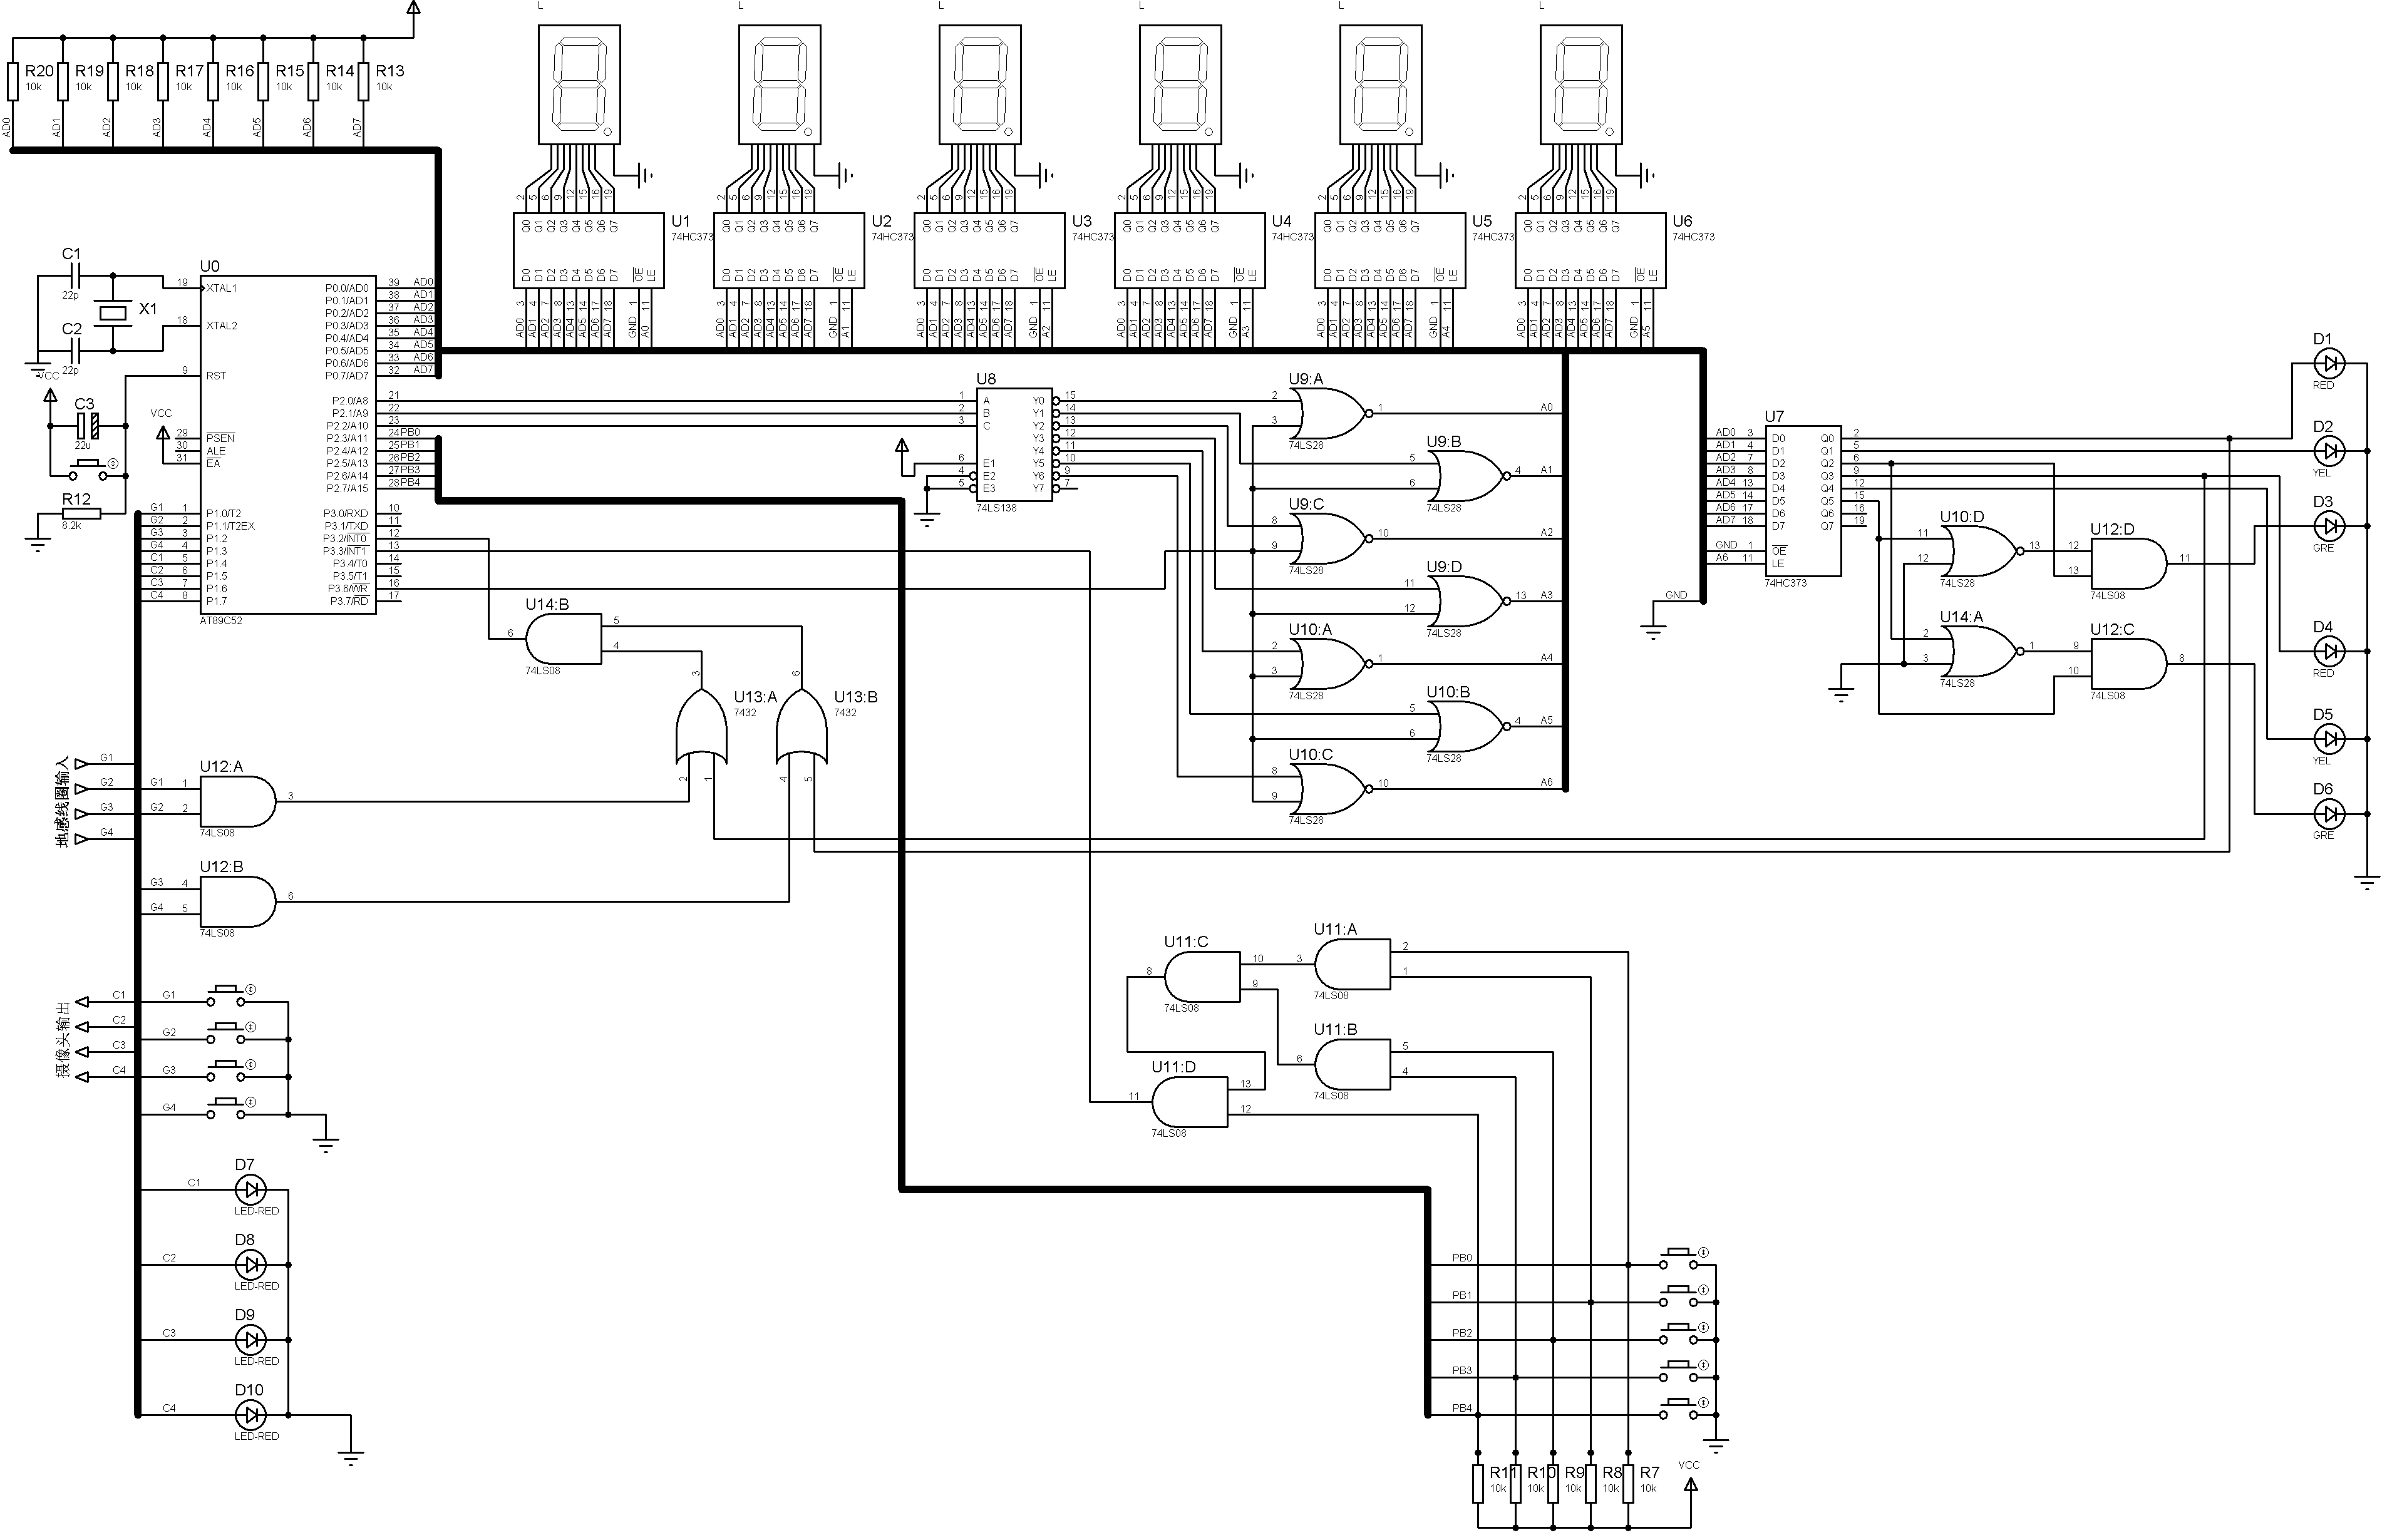
\includegraphics[width=0.85\textwidth]{chap2/circuitsmall.png}
  \bicaption[fig:circuitsmall]{电路图(小)}{控制电路图}{Fig}{Control Circuit Figure}
\end{figure}
	要实现规定的功能目标,通过估算,另外也考虑到S52单片机内部存储器足够大(8K),而最终生成的程序为1.32Kb,RAM空间也有剩余,故不需要进行存储器的扩展。
	
	地感线圈处的输入信号需通过继电器与控制电路连接,具体的连接参数视地感线圈而定。信号灯与数码管的控制信号需要通过光电耦合器后放大再驱动相应器件。这些电路,在以上的控制电路图中并没有体现,但在完整的系统中,它们是同样重要的。
	
\section{数码管及信号灯驱动电路}
	
	\subsection{数码管}
	数码管采用共阴数码管。为了提高显示质量,每一个数码管均通过一个373锁存器驱动,共六个。这样做可以实现静态显示,数码不会闪烁。软件实现也大为便捷,CPU占用率也降低许多。图\ref{fig:hard:digitled}是数码管部分的电路图。
	\begin{figure}[!tbh]
	\centering
	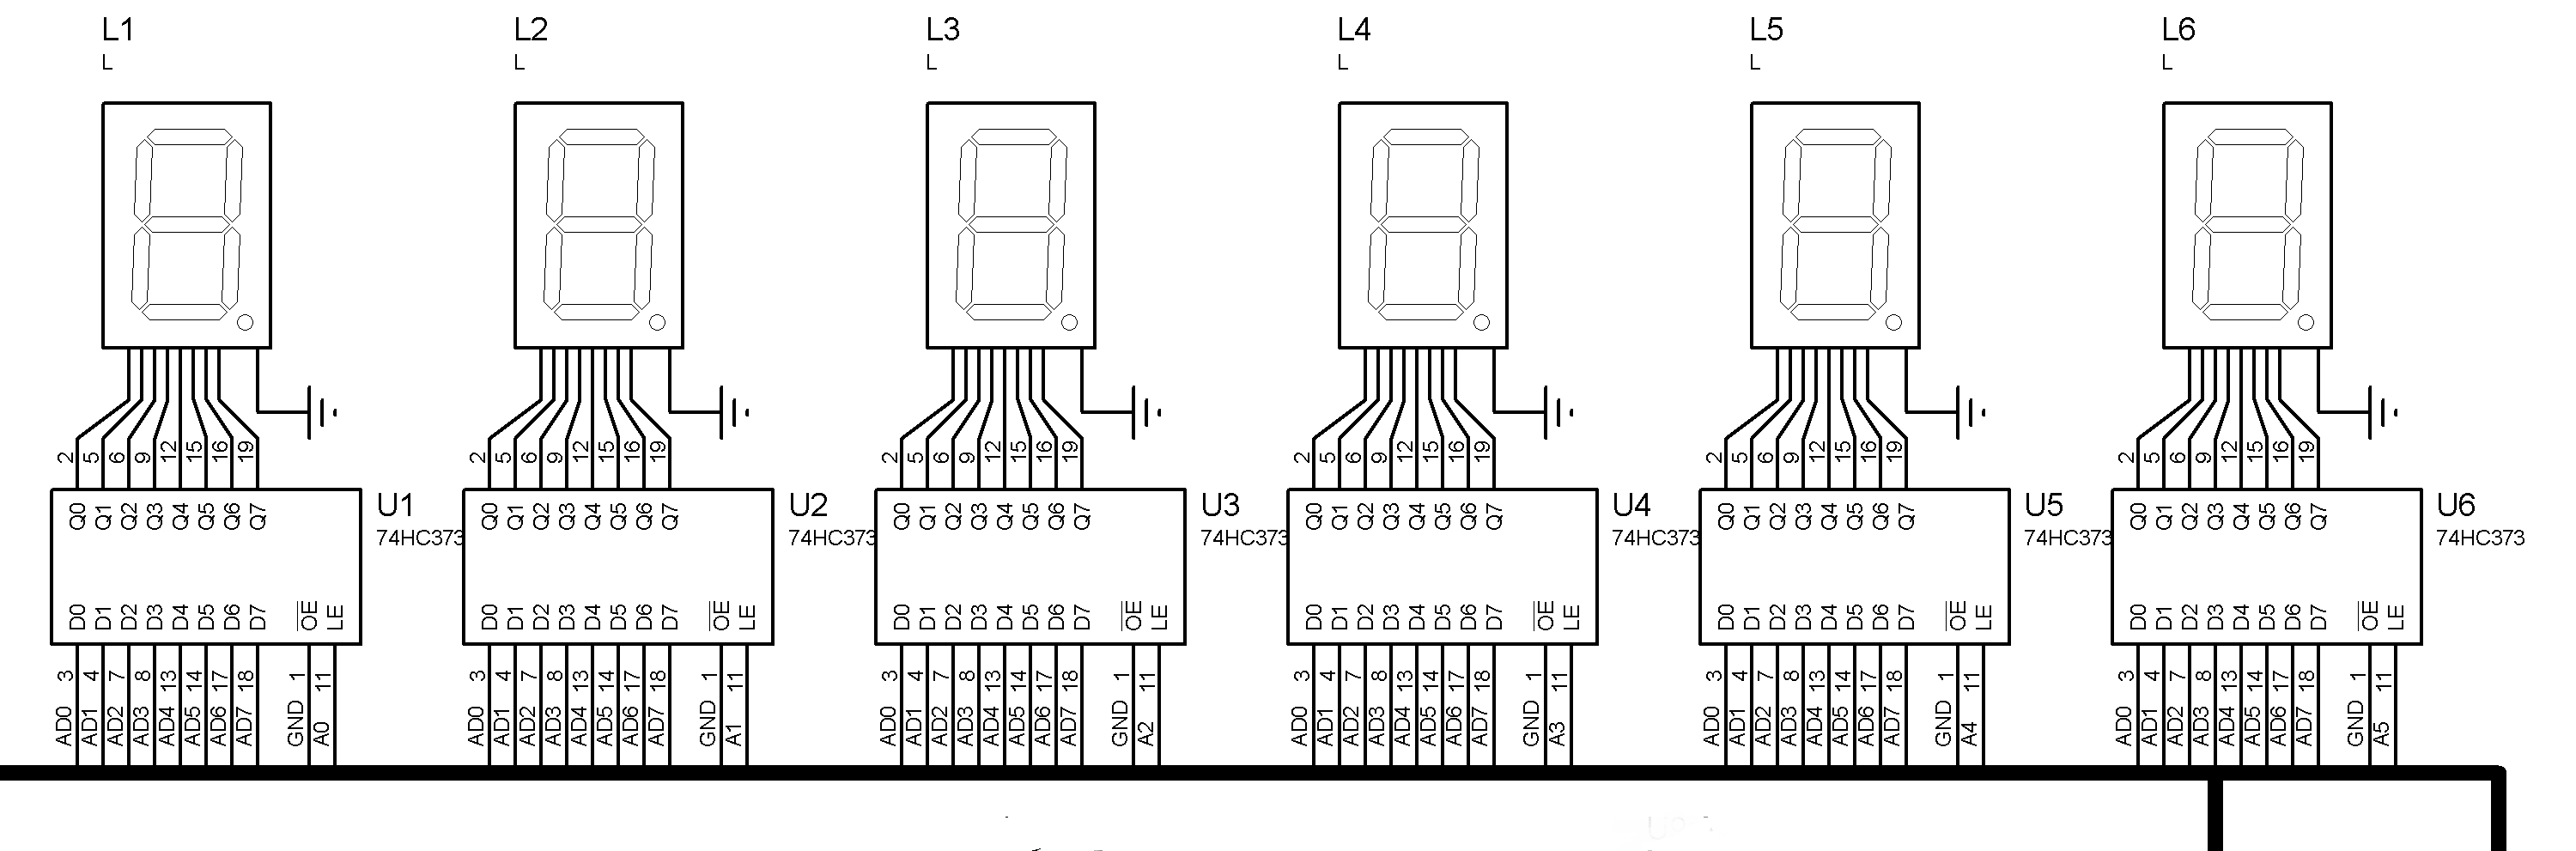
\includegraphics[width=0.7\textwidth]{chap2/digitled.png}
	\bicaption[fig:hard:digitled]{数码管驱动电路}{数码管驱动电路}{Fig}{Digital Led drive circuit}
	\end{figure}
	
	\subsection{信号灯驱动电路} \label{sec:hard:lightbull}
	信号灯驱动电路如图\ref{fig:hard:lightbull}所示。因为相对的路的信号灯内容相同,所以两条路且每条路三盏灯,共六盏灯,通过一个373锁存器驱动。图中可见互锁电路由两个或非门(非门)和两个与门组成,则两个绿灯不能同时点亮。尽管软件中避免了两盏绿灯同时点亮的情况的出现,但硬件互锁还是必不可少的,毕竟软件在运行过程中可能会受到干扰而混乱,可能出现不可预料的情况。
	
	图中所绘的小灯为演示所用,实际应将输出信号放大后,再驱动高电压的信号灯。
	\begin{figure}[!tbh]
	\centering
	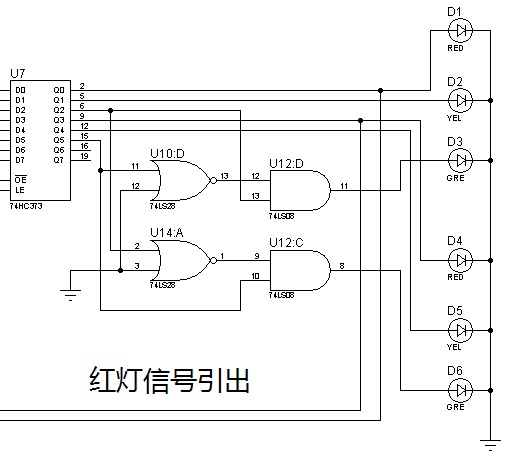
\includegraphics[width=0.6\textwidth]{chap2/lightbull.png}
	\bicaption[fig:hard:lightbull]{信号灯驱动电路}{信号灯驱动电路}{Fig}{Signal light drive circuit}
	\end{figure}
	
	图中还可以看到两个红灯处引出了两路信号,这样做的目的将在\ref{sec:hard:int0}节详细阐述。
	
	\subsection{数码管及信号灯的选通}
	P0口作为数据总线和七个373锁存器相连,P1口的低三位作为地址线,再经过一个38译码器选通各锁存器。单片机的WR信号与38译码器的七个输出端分别或非之后再选通锁存器。在对方案的重新评估中,我们发现也可以令WR信号直接选通138译码器,但考虑到译码器的输出端仍需通过非门,器件数量并未减少太多,故仍保留最初的设计。

\section{键盘}
	图\ref{fig:hard:keyboard}是键盘的电路图。因为P2口正好还有五个IO口可用,五个键也正好可以实现设置的要求,所以采用的独立键盘。这样对于编程工作也是很大的便利。各键的定义在\ref{sec:keydefination}节介绍。
	\begin{figure}[!tbh]
	\centering
	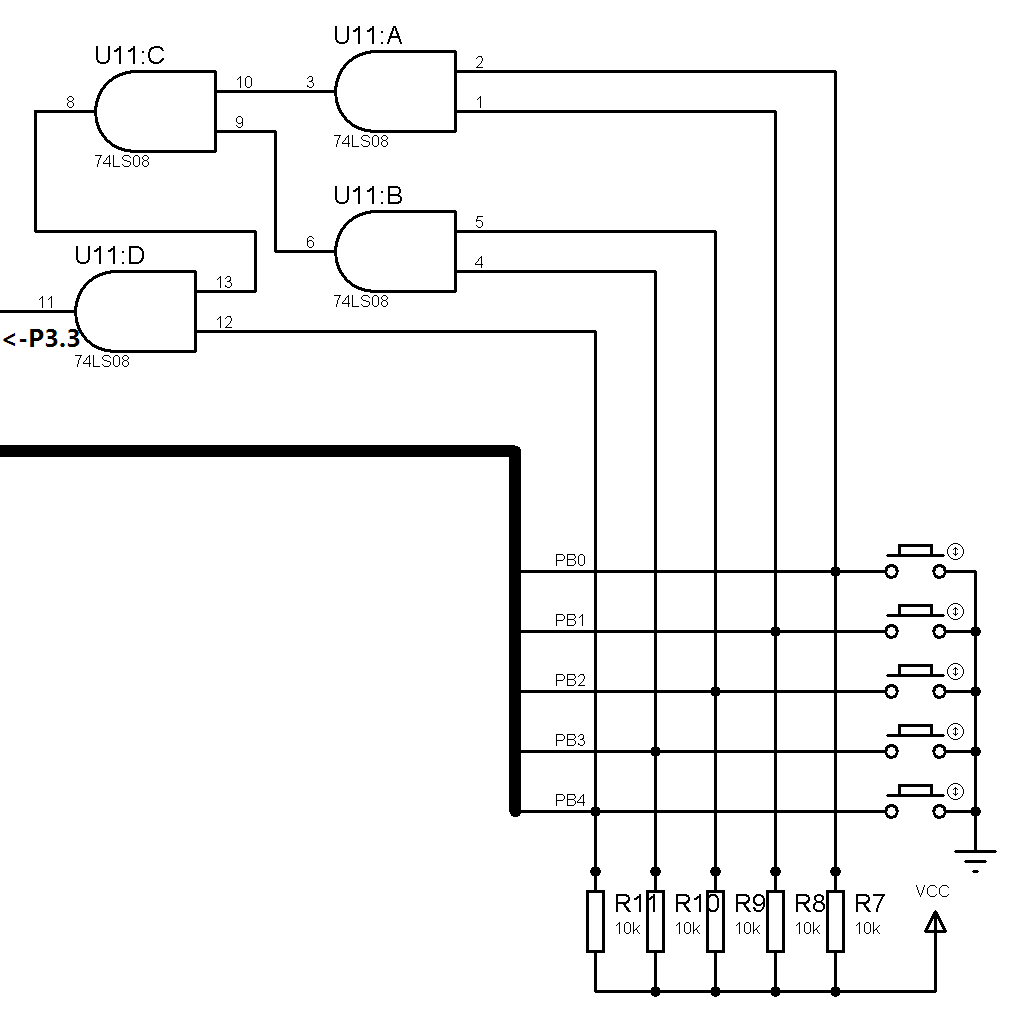
\includegraphics[width=0.5\textwidth]{chap2/keyboard.png}
	\bicaption[fig:hard:keyboard]{键盘电路}{键盘电路}{Fig}{Keyboard circuit}
	\end{figure}
	
	按键触发后P2口有下降沿信号,这个信号全部相与后接P3.3($\bf \overline{INT1}$),可产生中断信号,在软件中再通过轮询确定具体按下的键位。
	
\section{地感线圈输入与中断触发} \label{sec:hard:int0}
	地感线圈输入信号送入P1口低三位,并触发$\bf \overline{INT0}$中断。在电路图中地感线圈的输入以开关代替,实际信号也是一开关量,但由地感线圈转换至单片机控制电路输入信号还需要一些处理。
	
	\begin{figure}[!tbh]
	\centering
	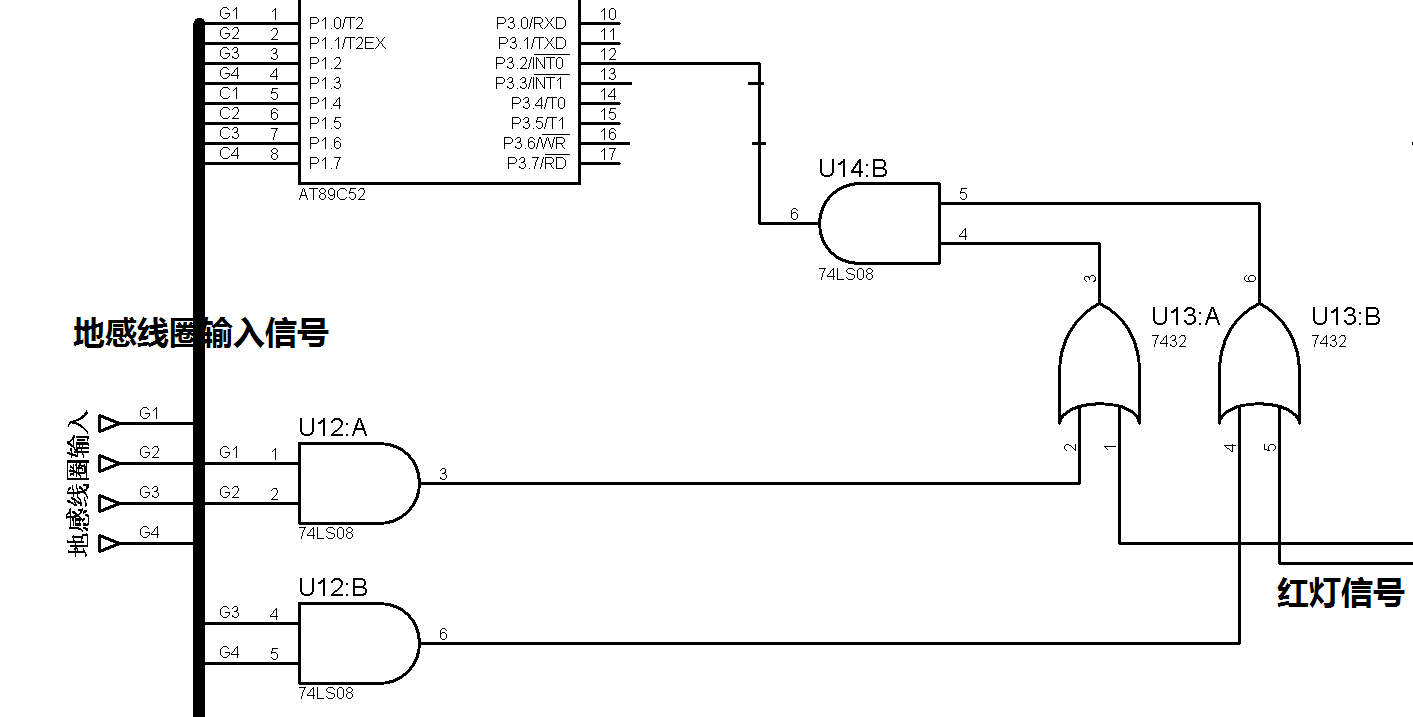
\includegraphics[width=0.7\textwidth]{chap2/redint0.png}
	\bicaption[fig:hard:redint0]{地感线圈输入电路}{地感线圈输入电路}{Fig}{Ground wire input}
	\end{figure}
	
	由图\ref{fig:hard:redint0}可见,此电路与普通的外部中断扩展电路稍有不同,在\ref{sec:hard:lightbull}节已提到,两路红灯信号由右侧引入,分别与另一条路的地感线圈输入信号取或运算,然后在送入$\bf \overline{INT0}$口。这是为了在某一路为绿灯时,屏蔽其地感线圈的信号,使之不能产生中断。只有在某一路为红灯时,闯红灯的车辆才能触发地感线圈,继而触发单片机中断。这样大大减少了中断的产生大大降低了CPU的工作量,提高了反映速度。编程难度也有所减轻。

\section{小结}
除了以上介绍的主要输入输出电路外,我们还设计了上电复位电路,晶振频率为11.0952MHz的时钟电路,P0口加入了上拉电阻。由于这些电路都较为常规,在此不再详述。

通过以上的分析可见,我们的设计对单片机IO口的利用非常充分P0,P1,P2口均已占满。通过充分利用IO口实现了数码管和信号灯的静态显示、独立键盘、独立的地感线圈输入,减少了元器件的使用,减小了编程难度。

硬件电路设计中也通过一些逻辑电路的组合,实现了互锁、条件屏蔽等功能。
%%==================================================
%% chapter03.tex for SJTU Course Design Thesis
%% based on CASthesis, SJTU master thesis
%% modified by icetiny@gmail.com
%% version: 0.3a
%% Encoding: UTF-8
%% last update: Dec 5th, 2010
%%==================================================

% \bibliographystyle{sjtu2} %[此处用于每章都生产参考文献]
\chapter{系统功能设计}
\label{chap:functionintro} 
	本章起到一个功能说明书的作用,将抛开底层的硬件和具体的软件实现,面向普通用户,介绍本系统的主要功能、工作流程,以及设置界面的使用方法。本章也作为下一章软件设计的先导,软件设计都是围绕着以下功能的实现而进行的。
	
	合理的硬件设计也是以下功能实现的重要基础。
\section{信号灯交替流程}
	红黄绿三色信号灯按照图\ref{fig:lightbullflow}所示的工作顺序交替闪亮。由于相交的两条路交通状况可能相差很大,其红灯持续时间是不同的。两个红灯时间T1和T2可以分别设置\footnote{下文将称这两个参数为亮灯时间参数},黄灯时间默认为3秒。由图可见一个亮灯循环只需要两个独立参数(T1和T2)就可以确定,绿灯时间比相应红灯时间短3秒。
	\begin{figure}[!tbh]
      \centering
      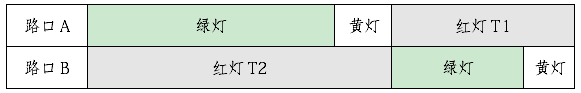
\includegraphics[width=0.9\textwidth]{chap3/lightbullflow.png}
      \bicaption[fig:lightbullflow]{亮灯顺序循环图}{亮灯顺序循环图}{Fig}{Signal light changing pattern}
    \end{figure}
    
	各个路口均悬挂有倒计时显示器,两组相对的路口显示内容分别相同。倒计时的内容为当前亮的灯将要持续的时间。当显示完\textbf{00}之后,灯的状态改变,倒计时显示屏也重新开始计数。 
	
\section{可调的亮灯时间}
所谓亮灯时间的可调性,就是指图\ref{fig:lightbullflow}中的循环参数T1和T2是可变的,这是为了适应不同的交通状况,车流量大时缓解拥堵,车流量小时减少等待。调节亮灯时间的方式有以下三种。
\subsection{预置数据表调节} 在单片机的ROM中预先存放了一数据表,一天中的每小时\footnote{一天中划分为24个时间段,从0到23,分别对应一天中的第一到第24个小时。}都有存储了两个数据在表中,分别代表A路口和B路口的红灯时间。则此表格共包含48个数据。单片机会根据当前的时间段\footnote{单片机复位后,用户可通过键盘设定初始时区为当前时间段,如图\ref{fig:keysetflow},之后单片机即从此时区开始自动累加},自动切换亮灯时间。
\subsection{用户自定义亮灯时间} 本系统还提供了一人机界面(包括5个按键和2位数显屏)供用户随时调节亮灯时间。用户可以调节任一时间段的亮灯时间,也可以重新定义当前所处的时间段。若用户调节了当前时间段的亮灯时间,则在当前红灯倒计时变为0后立即生效。\ref{sec:functionkeyboard}节会详细介绍该方式的使用方法。

时间参数存储在RAM中,单片机复位后会全部清零。用户定义的时间参数优先级比内置参数表高。
\subsection{双机通信调节} 单片机系统中留出了接口,上位机可以通过串行接口向单片机发出指令,直接改变当前时间段的亮灯时间参数。上位机可以是自动监控车流量的单片机,也可以是交通管理网络中的计算机。这种调节方式和通过键盘的调节方式,后设置的参数会覆盖之前覆盖的参数,所以它们的优先级是一致的。

\section{键盘屏显接口使用方法} \label{sec:functionkeyboard}
用户通过键盘可以实现两个功能。
\begin{enumerate}
\item 设定任一时段两路口的红灯时间参数,该参数存入RAM中。
\item 当用户设定的数据为两个00,则更改目前的时间区段为用户设定的值,这一功能可用于在单片机复位后初始化当前时区。
\end{enumerate}
在设定过程中,数字显示的相应位会闪烁,提示用户目前正在操作的位的位置。
\subsection{键位定义} \label{sec:keydefination}
		表\ref{tab:keydef}详细列出了各个按键的定义,了解了这张表基本就可以尝试操作了。但是由于屏显只有两位数码管,刚开始也许还会有些费解,还需要参考\ref{sec:keysetflow}节给出的一个完整的设置流程图。
		\begin{table}[!htpb]
      	\centering
      	\bicaption[tab:keydef]{键位定义}{键位定义}{Table}{keyboard defination}
      	\begin{tabular}{lcc|p{0.6\textwidth}} \toprule
        \multicolumn{2}{c}{键名} & 端口 & \multicolumn{1}{c}{功能} \\ \midrule
        开关 &on/off & p2.3 & 开关显示屏。开屏则首先显示当前时间段代码。关屏则重置键盘接口,清空所有寄存器。\\ \hline
        确认键&ok & p2.4 & 确认当前选择,并前进到下一选择界面\\ \hline
        选位键&<> & p2.5 &切换选择高低位。在设定数码时,用于在个位十位间切换,被选择的位会闪烁。设定时间段时,该键不起作用。\\ \hline
        加一键& + & p2.6 &使屏显的内容加一。在红灯时间调节状态下,对闪烁的位加一。若超出最大值,则变为最小值。\\ \hline
        减一键& -  & p2.7 &使屏显的内容减一。在红灯时间调节状态下,对闪烁的位减一。若小于最小值,则变为最大值。\\ 
				 \bottomrule
      	\end{tabular}
		\end{table}
\subsection{键盘设定操作流程}  \label{sec:keysetflow}
图\ref{fig:keysetflow} 是键盘相关的完整流程图。从图中可以明确看到,通过键盘设定可以完成两个功能。

需要补充的一点是,在成功设置某一时段的时间参数后,程序将检查设置的是否就是当前时段,如果是的话,会重新载入该时间常数。故更改会在当前红灯倒计时完毕后立即生效。
\begin{figure}[!tbhp]
      \centering
      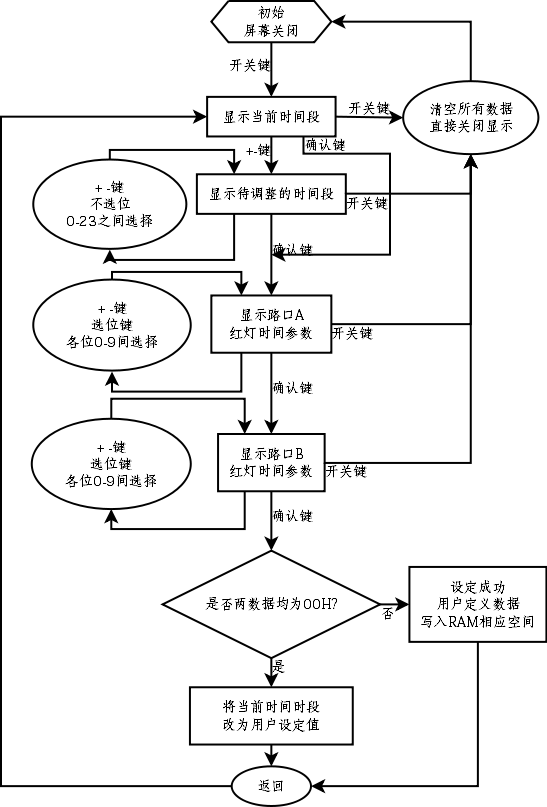
\includegraphics[width=0.85\textwidth]{chap3/keysetflow.png}
      \bicaption[fig:keysetflow]{键盘操作流程图}{键盘操作流程图}{Fig}{keyboard control flow figure}
    \end{figure}
\subsection{强壮性设计}
如果用户向信号灯系统定义了两个0为时间参数,显然这样的定义是没有意义的,通过软件已经将这样的输入转换为对当前时间段的重定义。本节就将讨论用户对用户各种输入数据的处理。

因为黄灯时间需要持续三秒,所以红灯时间必须大于3秒,任何小于三秒的定义也是无效的。
	\begin{table}[!htpb]
      	\centering
      	\bicaption[tab:keyresetmap]{键盘输入处理}{键盘输入处理}{Table}{keyboard input interpretation}
      	\begin{tabular}{c c |c c} \toprule
        \multicolumn{2}{c|}{用户输入}  &  \multicolumn{2}{c}{\multirow{2}*{相应处理}}  \\ \cmidrule(lr){1-2}   
        T1 & T2 \\ \cmidrule(lr){1-1}  \cmidrule(lr){2-2} \cmidrule(lr){3-4} 
        0 & 0 & \multicolumn{2}{c}{设置当前时间段} \\
        $\ge 0, <3$ & $\ge 0, <3$  & \multicolumn{2}{c}{无效输入,不操作}\\
        $\ge 0, <3$  & 有效输入T2 & T2 写入A路口对应RAM & T2 写入A路口对应RAM \\
        有效输入T1 & $\ge 0, <3$ & 写入T1 & 写入T1 \\
        有效输入T1 & 有效输入T2	& 写入T1 & 写入T2 \\ \bottomrule
      	\end{tabular}
		\end{table}

表\ref{tab:keyresetmap}列出了软件中对于各种输入情况的处理。由表可见,程序会自动消除用户的错误输入。默认的修正原则是:如果两个数据都错误则抛弃;如果其中有一个数据有效,则另一个路口的时间参数取相同的值。

\section{闯红灯拍照功能}
本系统还具有对闯红灯的车辆拍照的功能。需要说明的是,四个路口分别布置了地感线圈,只有在该路为红灯状态时,地感线圈发出的信号才有效。系统可以响应两个相对的路口同时闯红灯的状况,虽然这种情况的几率并不大。

\section{仍待加入的功能}
待完成
%%==================================================
%% chapter04.tex for SJTU Master Thesis
%% based on CASthesis
%% modified by wei.jianwen@gmail.com
%% version: 0.3a
%% Encoding: UTF-8
%% last update: Dec 5th, 2010
%%==================================================

% \bibliographystyle{sjtu2} %[此处用于每章都生产参考文献]

\chapter{常被问到和不常被问到的问题}
\label{chap:faq}

\subsubsection*{我是否能够自由使用这份模板}
是的,你可以爱咋用就咋用。拿去卖钱的话麻烦先通知我一声,我得先把里面的~Bugs~剔除干净。

\subsubsection*{我的论文是~Word~排版的,学校图书馆是不是只收~\LaTeX~排版的论文}
显然不是,Word~版肯定收。

\subsubsection*{我的论文是~\LaTeX~排版的,学校图书馆是不是只收~Word~排版的论文}
显然不是,PDF~版的电子论文也是可以上交的。是否要交~Word~版就看你导师的喜好了。

\subsubsection*{为什么左右页边距不一样}
模板默认是双面打印,迎面页和背面页的页边距是要交换的,多出来的那一部分是留作装订的。

\subsubsection*{为什么在参考文献中会有``//''符号}
那是国标~GBT7714~参考文献风格规定的,如果下次有人怀疑``//''不合规范,你可以鄙视TA了。

\subsubsection*{为什么参考文献中会有[s.n.],[S.l], [EB/OL]等符号}
那也是国标~GBT7714~参考文献风格定义的。[s.n.]表示出版者不祥,[S.l]表示出版地不祥,[EB/OL]表示引用的参考文献类型为在线电子文档。

\subsubsection*{如何获得帮助和反馈意见}
你可以通过查看文档、到TeX\_LaTeX版发帖来获得帮助。如果你觉得你的意见足够高明,可以直接给我\href{mail:wei.jianwen@gmail.com}{发邮件}。

\subsubsection*{你做这个是有偿劳动吗}
我做这个模板是无偿劳动。

\subsubsection*{如何向你表示感谢}
口头感谢、站内感谢、\href{wei.jianwen@gmail.com}{MSN感谢}、送锦旗、请吃饭、写入你论文致谢都可以,但最好你能帮我解决第\ref{chap:needsomehelp}章中的问题。谢谢大家。


%%%==================================================
%% conclusion.tex for SJTU Master Thesis
%% based on CASthesis
%% modified by wei.jianwen@gmail.com
%% version: 0.3a
%% Encoding: UTF-8
%% last update: Dec 5th, 2010
%%==================================================

\chapter*{全文总结\markboth{全文总结}{}}
\addcontentsline{toc}{chapter}{全文总结}

这里是全文总结内容。

 %% 全文总结


%%%%%%%%%%%%%%%%%%%%%%%%%%%%%% 
%% 附录(章节编号重新计算,使用字母进行编号)
%%%%%%%%%%%%%%%%%%%%%%%%%%%%%% 
\appendix

% 附录中编号形式是"A-1"的样子
\renewcommand\theequation{\Alph{chapter}--\arabic{equation}}
\renewcommand\thefigure{\Alph{chapter}--\arabic{figure}}
\renewcommand\thetable{\Alph{chapter}--\arabic{table}}

%%%==================================================
%% app1.tex for SJTU Master Thesis
%% based on CASthesis
%% modified by wei.jianwen@gmail.com
%% version: 0.3a
%% Encoding: UTF-8
%% last update: Dec 5th, 2010
%%==================================================

\chapter{源程序}
\label{app:code}
\begin{lstlisting}[language={[x86masm]assembler},  escapeinside=""]
;;------------------------
;;TrafLight v2.0
;;by SN icetiny@gmail.com
;;2011-6-16
;;------------------------
;;\verb+R0 | R1 | R2| R3+
;;\verb+灯状态 | 临时使用 | 2红灯倒计时 | 1绿灯倒计时+    
;;\verb+	R6  |  R7  |  R5+		
;;\verb+秒状态数码 | 分状态| 空+
;;\verb+   R4  +
;;\verb+屏状态(0开1选段2调路口A3调路口B)+
;;------------------------
;;\verb+30H  |  31H  |  32H-35H  |  36H  |  37H+
;;\verb+红灯A | 红灯B | 灯状态地址 | 减一用 | 当前小时状态码+
;;------------------------
;;\verb+		38H  |  39H  |  3AH  |  3BH  |  3CH+	
;;\verb+LED显示寄存器 | 数码管地址高八位 | 屏段(HEX码) | 屏绿灯 | 屏红灯+
;;------------------------
;;\verb+		位7F  |  3DH  |  3EH+
;;\verb+选位标志 | BCDINC和BCDDEC子程序的操作位 | 闪烁关灯程序数据传递位+
;;------------------------
;;\verb+50H-7FH  |  40H 41H  |  位7E+
;;\verb+用户定义灯状态 | delay10中用到的变量 | 区分一秒中的上下半秒+
;;------------------------
;;键盘
;;\verb+1  |  2  |  3  |  4  |  5+
;;\verb+on/off | ok/next | <>选位 | +  - +
;;------------------------

		ORG 0000H
		AJMP MAIN
;----------------INTERRUPT VECTORS--------------------------
		ORG 0003H ;外部中断0
		LJMP INT_EX0
		ORG 000BH							
		LJMP INT_TO							
		ORG 0013H ;外部中断1						
		LJMP INT_EX1							
		ORG 001BH							
		LJMP INT_C1							
;------------DEFINE CONSTANT VALUE--------------------------
		LDD1 EQU 0f8H ;数码管地址
		LDD2 EQU 0f9H
		LDD3 EQU 0faH
		LDD4 EQU 0fbH
		LDD5 EQU 0fcH
		LDD6 EQU 0fdH
		LED  EQU 0feH ;灯地址
		G_R1 EQU 1100B
		Y_R2 EQU 1010B
		R_G3 EQU 100001B
		R_Y4 EQU 10001B
		SECS_PER_MIN EQU 4  ;每分中的秒数,调试用
		MINS_PER_HOUR EQU 5 ;每小时中的分数,调试用																							
;-----------------------------------------------------------	
;;--------------MAIN PROGRAM BEGIN---------------------------
		ORG 0030H				 
MAIN:	
		MOV SP,#10H
		MOV P1,#0FH
		MOV 32H,#G_R1
		MOV 33H,#Y_R2
		MOV 34H,#R_G3
		MOV 35H,#R_Y4
		MOV TMOD,#61H	;初始化计时器 定时器0方式1 计数器1方式2
		MOV TH0,#0E7H	
		MOV TL0,#09H	;$2^{16}-6400 = 59136 = E700$, $E700+7=E707$
		;$12*2*72*6400=11.0592MHz$,取得较小是为了照顾WDT看门狗
		MOV TH1,#0DCH
		MOV TL1,#0DCH	;36. 0.5S ;	
		MOV R6,#SECS_PER_MIN ;每分中的秒数,调试用
		MOV R7,#MINS_PER_HOUR ;每小时中的分数,调试用
		MOV 37H,#8		;初始化当前时间(小时状态)
		LCALL GET_LIGHT_TIME ;获取倒计时时间存入 30H,31H
		MOV R0,#32H	;R0记录信号灯寄存器状态
		MOV R2,30H
		MOV R3,30H
		MOV 36H,R3
		LCALL SUBBCD
		LCALL SUBBCD
		LCALL SUBBCD
		MOV R3,36H
		LCALL CHANGE_LIGHT	;开信号灯
		MOV 38H,R3	   ;送显示,开数码管
		MOV 39H,#LDD2
		LCALL DISPLAY_NUMBER
		MOV 38H,R2
		MOV 39H,#LDD4
		LCALL DISPLAY_NUMBER
		;中断优先级处理
		MOV IP,#00001010B	 ;优先级依次为 t0 t1 x0 x1
		MOV IE,#10001111B	 ; \verb+EA | - | ET2 | ES | ET1 | EX1 | ET0 | EX0+
						 ; \verb+1 | 0 | 0 | 0 | 1 | 1 | 1 | 1+
		MOV TCON,#05H		 ;IT0=1 IT1=1
		SETB TR0			 ;开定时器
		SETB TR1
		MOV 0A6H,#01EH ;激活看门狗
		MOV 0A6H,#0E1H 
		;初始化完毕,开始计时
		SJMP "\$"
;;-------------- END OF MAIN -----------------
INT_TO:								;计时器0中断处理程序
		nop
		MOV TH0,#0E7H 				
		MOV TL0,#09H
		MOV 0A6H,#01EH 				;清零看门狗
		MOV 0A6H,#0E1H 
		CPL P3.5
		RETI
		
INT_C1:								;计数器1中断处理程序
		PUSH ACC
		CPL 7EH
		JB 7EH,INT_C1_NORMAL
INT_C1_BLINK:
		MOV A,R4
		JZ INT_C1_BLINK_EXIT		
		MOV A,R4
		CLR C
		SUBB A,#2
		JBC CY,INT_C1_BLINK_EXIT
		JNZ INT_C1_BLINK_RED
		MOV 3EH,3BH
		LCALL CLOSEDIG
		LJMP INT_C1_EXIT1
INT_C1_BLINK_RED:
		MOV 3EH,3CH
		LCALL CLOSEDIG		
INT_C1_BLINK_EXIT:
		LJMP INT_C1_EXIT1				
INT_C1_NORMAL:
		MOV A,R4
		JZ INT_C1_NORMAL1		
		MOV A,R4
		CLR C
		SUBB A,#2
		JBC CY,INT_C1_NORMAL1
		JNZ INT_C1_UNBLINK_RED
		MOV 38H,3BH
		MOV 39H,#LDD6
		LCALL DISPLAY_NUMBER
		LJMP INT_C1_NORMAL1
INT_C1_UNBLINK_RED:
		MOV 38H,3CH
		MOV 39H,#LDD6
		LCALL DISPLAY_NUMBER				
INT_C1_NORMAL1:		MOV 36H,R3
		LCALL SUBBCD
		MOV R3,36H
		MOV 36H,R2
		LCALL SUBBCD
		MOV R2,36H
		CJNE R2,#0F9H,INT_C1_NEXT2
		INC R0
		CJNE R0,#36H,INT_C1_NEXT0
		MOV R0,#32H
		LCALL CHANGE_LIGHT
		MOV R2,30H
		MOV R3,30H	   ;绿灯时间比红灯时间短3秒
		MOV 36H,R3
		LCALL SUBBCD
		LCALL SUBBCD
		LCALL SUBBCD
		MOV R3,36H
		SJMP INT_C1_EXIT
INT_C1_NEXT0:
		CJNE R0,#34H,INT_C1_NEXT1
		LCALL CHANGE_LIGHT
		MOV R2,31H
		MOV R3,31H	   ;绿灯时间比红灯时间短3秒
		MOV 36H,R3
		LCALL SUBBCD
		LCALL SUBBCD
		LCALL SUBBCD
		MOV R3,36H
		SJMP INT_C1_EXIT
INT_C1_NEXT1:
		CJNE R0,#35H,INT_C1_NEXT2
		LCALL CHANGE_LIGHT
		MOV A,R3
		XCH A,R2
		SJMP INT_C1_EXIT
INT_C1_NEXT2:
		CJNE R3,#0F9H,INT_C1_EXIT
		INC R0
		LCALL CHANGE_LIGHT
		MOV A,R2
		XCH A,R3
INT_C1_EXIT:
		MOV A,R0
		CLR CY
		SUBB A,#33H
		JNB CY,INT_C1_REVERSEDISPLAY
		MOV 38H,R3	   ;送显示
		MOV 39H,#LDD2
		LCALL DISPLAY_NUMBER
		MOV 38H,R2
		MOV 39H,#LDD4
		LCALL DISPLAY_NUMBER
		LJMP INT_C1_EXIT00
INT_C1_REVERSEDISPLAY:	;调换显示的内容(原来显示红灯倒计时,现在则显示绿灯倒计时)
		MOV 38H,R2	   
		MOV 39H,#LDD2
		LCALL DISPLAY_NUMBER
		MOV 38H,R3
		MOV 39H,#LDD4
		LCALL DISPLAY_NUMBER
INT_C1_EXIT00:
		DJNZ R6,INT_C1_EXIT1
		MOV R6,#SECS_PER_MIN
		DJNZ R7,INT_C1_EXIT1
		MOV R7,#MINS_PER_HOUR
		INC 37H
		MOV A,37H
		CJNE A,#24,INT_C1_EXIT0
		MOV 37H,#0
INT_C1_EXIT0:
		LCALL GET_LIGHT_TIME
INT_C1_EXIT1:
		POP ACC
		RETI
;-------------地感线圈中断处理----------------
INT_EX0:
		PUSH ACC
		MOV A,P1
					CJNE R0,#32H,INT_EX0_NEXT1
					LJMP INT_EX0_SHOOT2
INT_EX0_NEXT1:		CJNE R0,#33H,INT_EX0_NEXT2
					LJMP INT_EX0_SHOOT2
INT_EX0_NEXT2:		CJNE R0,#34H,INT_EX0_NEXT3
					LJMP INT_EX0_SHOOT1
INT_EX0_NEXT3:		CJNE R0,#35H,INT_EX0_EXIT
INT_EX0_SHOOT1:		JB ACC.0,INT_EX0_SHOOT11
					SETB P1.4
INT_EX0_SHOOT11:
					JB ACC.1,INT_EX0_EXIT
					SETB P1.5
					LJMP INT_EX0_EXIT
INT_EX0_SHOOT2:		JB ACC.2,INT_EX0_SHOOT22
					SETB P1.6
INT_EX0_SHOOT22:
					JB ACC.3,INT_EX0_EXIT
					SETB P1.7
INT_EX0_EXIT:
		MOV A,#30
INT_EX0_EXIT0:
		LCALL DELAY10
		DJNZ ACC,INT_EX0_EXIT0
INT_EX0_EXIT1:
		MOV P1,#0FH
		POP ACC
		RETI
;-------------按键中断处理程序----------------
INT_EX1:							;外部中断1处理,键盘
		PUSH PSW
		PUSH ACC
		MOV A,P2   ;判断是否有键按下
		ANL A,#0F8H
		XRL A,#0F8H
		JZ INT_EX1_EXIT 
		LCALL DELAY10
		MOV A,P2   ;再次判断是否有键按下,消除前沿抖动
		ANL A,#0F8H
		XRL A,#0F8H
		JZ INT_EX1_EXIT
		JB ACC.3,KEY01
		JB ACC.4,KEY02
		JB ACC.5,KEY03
		JB ACC.6,KEY04
		JB ACC.7,KEY05
		KEY01:LJMP KEY1
		KEY02:LJMP KEY2		
		KEY03:LJMP KEY3
		KEY04:LJMP KEY4
		KEY05:LJMP KEY5
INT_EX1_EXIT:
		MOV A,P2   ;判断是否有键按下,消除后沿抖动
		ANL A,#0F8H
		XRL A,#0F8H
		JZ INT_EX1_EXIT_1
		LCALL DELAY4ms5
		SJMP INT_EX1_EXIT
INT_EX1_EXIT_1:
		POP ACC
		POP PSW
		RETI

KEY1: ;开关键
		CJNE R4,#00,KEY1_NEXT1
		MOV R4,#1		 ;开启屏
		MOV 3AH,37H 
		MOV 38H,3AH
		LCALL HEX2BCD
		MOV 39H,#LDD6
		LCALL DISPLAY_NUMBER
		LJMP INT_EX1_EXIT
KEY1_NEXT1:
		MOV R4,#0		 ;关闭屏  
		MOV 3AH,#0
		MOV 3BH,#0
		MOV 3CH,#0
		MOV 38H,#0FFH
		MOV 39H,#LDD6
		LCALL DISPLAY_NUMBER 
		LJMP INT_EX1_EXIT

KEY2:	;确认键,OK键
		MOV A,R4
		MOV R1,A
		CJNE R1,#0,KEY2_R01
 		LJMP INT_EX1_EXIT
KEY2_R01:		DJNZ R1,KEY2_R02
				LJMP KEY2_R1
KEY2_R02:		DJNZ R1,KEY2_R03
				LJMP KEY2_R2
KEY2_R03:		DJNZ R1,INT_EX1_EXIT
				LJMP KEY2_R3
KEY2_R1:
		INC R4
		MOV 38H,3BH
		MOV 39H,#LDD6
		LCALL DISPLAY_NUMBER
		LJMP INT_EX1_EXIT
KEY2_R2:
		INC R4
		MOV 38H,3CH
		MOV 39H,#LDD6
		LCALL DISPLAY_NUMBER
		LJMP INT_EX1_EXIT
KEY2_R3:
		MOV R4,#1
		MOV 38H,3AH
		LCALL HEX2BCD
		MOV 39H,#LDD6
		LCALL DISPLAY_NUMBER
		MOV A,3AH
		RL A
		ADD A,#50H
		XCH A,R1
		MOV A,3BH
		CLR CY
		SUBB A,#3
		JNB CY, KEY2_R3_NEXT1
		MOV 3BH,#00H
KEY2_R3_NEXT1:
		MOV @R1,3BH
		INC R1
		MOV A,3CH
		CLR CY
		SUBB A,#3
		JNB CY, KEY2_R3_NEXT2
		MOV 3CH,#00H
KEY2_R3_NEXT2:
		MOV @R1,3CH 
		MOV 3BH,#00H
		MOV 3CH,#00H
		MOV R1,3AH	;如果更改的为当前时间段
				;则立即调用 GET\_LIGHT\_TIME 重载倒计时时间
		MOV A,37H
		CLR CY
		SUBB A,R1
		CJNE A,#00H,KEY2_R3_EXIT
		LCALL GET_LIGHT_TIME
KEY2_R3_EXIT:
		LJMP INT_EX1_EXIT

KEY3:	CPL 7FH						;选位数
		LJMP INT_EX1_EXIT

KEY4:			         ;加一
		MOV A,R4		
		MOV R1,A
		CJNE R1,#0,KEY4_R01
 		LJMP INT_EX1_EXIT
KEY4_R01:		DJNZ R1,KEY4_R02
				INC 3AH
				MOV A,3AH
				CJNE A,#24,KEY4_R01_next
				MOV 3AH,#0
KEY4_R01_next:	MOV 38H,3AH
				LCALL HEX2BCD
				MOV 39H,#LDD6
				LCALL DISPLAY_NUMBER
				LJMP INT_EX1_EXIT
KEY4_R02:		DJNZ R1,KEY4_R03
				MOV 3DH,3BH
				LCALL BCDINC
				MOV 3BH,3DH
				MOV 38H,3BH
				MOV 39H,#LDD6
				LCALL DISPLAY_NUMBER
				LJMP INT_EX1_EXIT
KEY4_R03:		DJNZ R1,KEY4_EXIT
				MOV 3DH,3CH
				LCALL BCDINC
				MOV 3CH,3DH
				MOV 38H,3CH
				MOV 39H,#LDD6
				LCALL DISPLAY_NUMBER
KEY4_EXIT:		LJMP INT_EX1_EXIT				  		

KEY5: 			MOV A,R4		;减一
				MOV R1,A
				CJNE R1,#0,KEY5_R01
 				LJMP INT_EX1_EXIT
KEY5_R01:		DJNZ R1,KEY5_R02
				MOV A,3AH
				CJNE A,#0,KEY5_R01_next
				MOV 3AH,#24
KEY5_R01_next:	DEC 3AH
				MOV 38H,3AH
				LCALL HEX2BCD
				MOV 39H,#LDD6
				LCALL DISPLAY_NUMBER
				LJMP INT_EX1_EXIT
KEY5_R02:		DJNZ R1,KEY5_R03
				MOV 3DH,3BH
				LCALL BCDDEC
				MOV 3BH,3DH
				MOV 38H,3BH
				MOV 39H,#LDD6
				LCALL DISPLAY_NUMBER
				LJMP INT_EX1_EXIT
KEY5_R03:		DJNZ R1,KEY5_EXIT
				MOV 3DH,3CH
				LCALL BCDDEC
				MOV 3CH,3DH
				MOV 38H,3CH
				MOV 39H,#LDD6
				LCALL DISPLAY_NUMBER
KEY5_EXIT:		LJMP INT_EX1_EXIT

BCDINC:	PUSH ACC
		MOV A,3DH
		JB 7FH,BCDINC_HIGH
		ANL A,#0FH
		CJNE A,#09H,BCDINC_LOW1
		ANL 3DH,#0F0H
		LJMP BCDINC_EXIT
BCDINC_LOW1:
		INC 3DH
		LJMP BCDINC_EXIT
BCDINC_HIGH:
		ANL A,#0F0H
		CJNE A,#90H,BCDINC_HIGH1
		ANL 3DH,#0FH
		LJMP BCDINC_EXIT
BCDINC_HIGH1:
		MOV A,3DH
		ADD A,#10H
		MOV 3DH,A
BCDINC_EXIT:		
		POP ACC
		RET
		
BCDDEC:	PUSH ACC
		MOV A,3DH
		JB 7FH,BCDDEC_HIGH
		ANL A,#0FH
		CJNE A,#00H,BCDDEC_LOW1
		ORL 3DH,#09H
		LJMP BCDDEC_EXIT
BCDDEC_LOW1:
		DEC 3DH
		LJMP BCDDEC_EXIT
BCDDEC_HIGH:
		ANL A,#0F0H
		CJNE A,#00H,BCDDEC_HIGH1
		ORL 3DH,#90H
		LJMP BCDDEC_EXIT
BCDDEC_HIGH1:
		MOV A,3DH
		SUBB A,#10H
		MOV 3DH,A
BCDDEC_EXIT:
		POP ACC	
		RET

CLOSEDIG:				;根据选位标志,关闭某一位的现实,实现闪烁功能
		PUSH ACC
		MOV A,3EH
		JB 7FH,CLOSEDIG_HIGH
		ORL A,#0FH
		LJMP CLOSEDIG_EXIT
CLOSEDIG_HIGH:
		ORL A,#0F0H
CLOSEDIG_EXIT:		
		MOV 38H,A
		MOV 39H,#LDD6
		LCALL DISPLAY_NUMBER
		POP ACC
		RET
;-------------END OF 按键中断处理程序----------------

HEX2BCD:			  ;将38H中的16进制数转为BCD码
		PUSH ACC
		MOV A,38H
		MOV B,#10
		DIV AB
		SWAP A
		ORL A,B
		MOV 38H,A
		POP ACC
		RET
;---------------------------
GET_LIGHT_TIME:							;获取当前红灯时间子程序,存入30h和31h
		PUSH DPH						;默认红灯时间大于3秒
		PUSH DPL
		PUSH ACC
		PUSH PSW
		SETB RS0		         
		MOV DPTR,#TAB_LIGHT_TIME ;读入信号灯延时信息,30H为红灯A,31H为红灯B
		MOV A,37H
		RL A
		MOVC A,@A+DPTR
		MOV 30H,A
		MOV A,37H
		RL A
		INC A
		MOVC A,@A+DPTR
		MOV 31H,A	
		;检查是否有用户自定义数据
		MOV A,37H
		RL A
		ADD A,#50H
		MOV R0,A
		INC A
		MOV R1,A
		MOV A,@R0  
		ORL A,@R1
		JZ GET_LIGHT_TIME_EXIT ;若全为零,说明无用户定义数据,直接跳出
		CJNE @R0,#00H,GET_LIGHT_TIME_NEXT1
		MOV 30H,@R1			   ;若只有一个为0,则使两路口数字相等
		AJMP GET_LIGHT_TIME_NEXT2
GET_LIGHT_TIME_NEXT1:
		MOV 30H,@R0
GET_LIGHT_TIME_NEXT2:
		CJNE @R1,#00H,GET_LIGHT_TIME_NEXT3
		MOV 31H,@R0
		AJMP GET_LIGHT_TIME_EXIT
GET_LIGHT_TIME_NEXT3:
		MOV 31H,@R1
GET_LIGHT_TIME_EXIT:
		CLR RS0
		POP PSW
		POP ACC
		POP DPL
		POP DPH
		RET
;--------------------
CHANGE_LIGHT:				;开信号灯子程序
		PUSH DPH
		PUSH ACC
		MOV DPH,#LED
		MOV A,@R0
		MOVX @DPTR,A
		POP ACC
		POP DPH
		RET
;-------------------------
DISPLAY_NUMBER:				;显示倒计时数字子程序,显示38H中的数字到39H指定的地址中 先显示低位,再显示高位
		PUSH ACC
		MOV A,38H
		ANL 38H,#0FH
		LCALL GETDIGIT
		MOV DPH,39H
		LCALL DISDIGIT
		SWAP A
		MOV 38H,A
		ANL 38H,#0FH
		LCALL GETDIGIT
		DEC 39H
		MOV DPH,39H
		LCALL DISDIGIT
		POP ACC
		RET
;-----------------------------
GETDIGIT:					;取段码子程序
		PUSH DPH
		PUSH DPL
		PUSH ACC
		MOV DPTR,#DIGIT
		MOV A,38H
		MOVC A,@A+DPTR
		XCH A,38H
		POP ACC
		POP DPL
		POP DPH
		RET
;--------------------------------				
DISDIGIT:					;送数码管显示子程序
		PUSH ACC
		MOV	A,38H
		MOVX @DPTR,A
		POP ACC 
		RET
;------------------------------
SUBBCD:						;BCD码减一,对36H中的数做BCD码减1
		PUSH ACC
		PUSH PSW
		DEC 36H
		MOV A,36H
		ANL A,#0FH
		CJNE A,#0FH,SUBBCD_EXIT
		CLR CY
		MOV A,36H
		SUBB A,#06
		MOV 36H,A
SUBBCD_EXIT:
		POP PSW
		POP ACC
		RET

DELAY10:
		NOP
		MOV 40H,#9
DL10_1: MOV 41H,#255
DL10_2: NOP
		NOP
		DJNZ 41H,DL10_2
		DJNZ 40H,DL10_1
		NOP
		RET

DELAY4ms5:
		MOV 40H,#4
DL45_1: MOV 41H,#210
DL45_2: NOP
		NOP
		NOP
		DJNZ 41H,DL45_2
		DJNZ 40H,DL45_1
		NOP
		RET
;;------------TABLES----------------			                 
DIGIT:							;LED数码管段码表
		DB 3FH,06H,5BH,4FH,66H
		DB 6DH,7DH,07H,7FH,6FH
		DB 77H,7CH,39H,5EH,79H,00H
TAB_LIGHT_TIME:  				;预设的信号灯时间常数,共24行,48个值
		DB 03H, 04H
		DB 04H, 05H
		DB 05H, 06H
		DB 06H, 07H
		DB 07H, 08H
		DB 08H, 09H
		DB 09H, 10H
		DB 10H, 11H
		DB 11H, 12H
		DB 12H, 13H
		DB 13H, 14H
		DB 14H, 15H
		DB 15H, 16H
		DB 16H, 17H
		DB 17H, 18H
		DB 18H, 19H
		DB 19H, 20H
		DB 20H, 21H
		DB 21H, 22H
		DB 22H, 23H
		DB 23H, 24H
		DB 24H, 25H
		DB 25H, 26H
		DB 26H, 27H
;----------- END --------------------
END
\end{lstlisting}

 % 源代码
%% app2.tex for SJTU Master Thesis
%% based on CASthesis
%% modified by wei.jianwen@gmail.com
%% version: 0.3a
%% Encoding: UTF-8
%% last update: Dec 5th, 2010
%%==================================================

\chapter{电路图}
\label{app:circuit}
\begin{figure}[!bh]
  \centering
  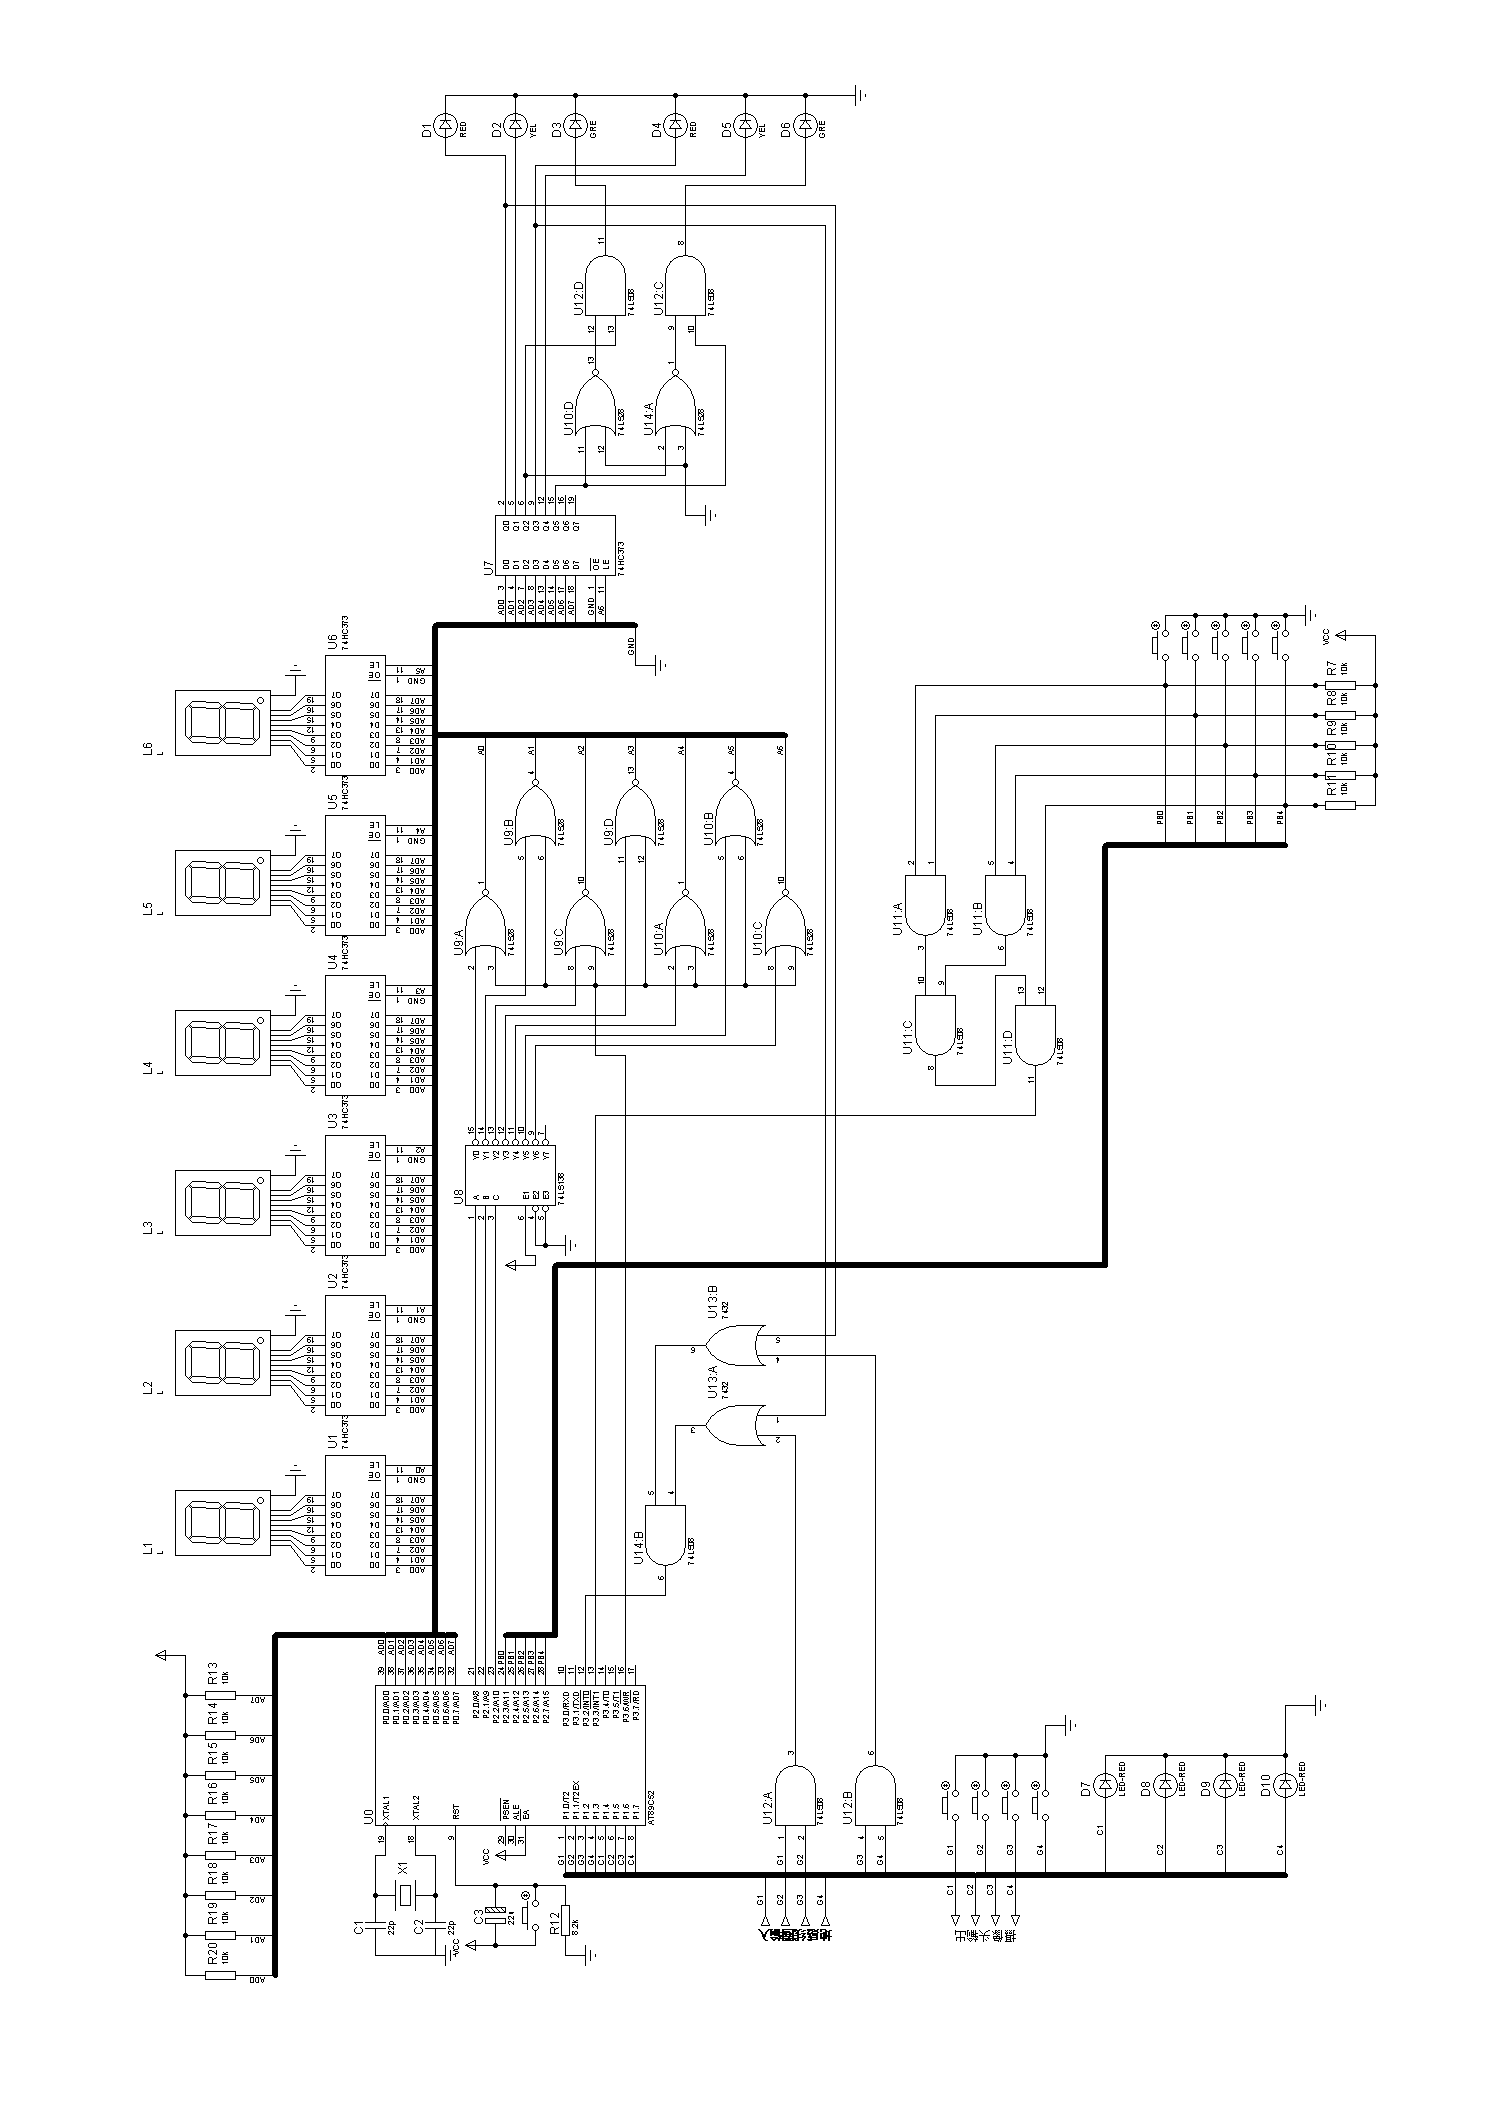
\includegraphics[origin=c, angle= -90,width=0.73\textwidth]{app2/circuitpng.png}
  \bicaption[fig:circuitall]{电路图}{电路图}{Fig}{Circuit Map}
\end{figure}


 %电路图


%%%%%%%%%%%%%%%%%%%%%%%%%%%%%% 
%% 文后(无章节编号)
%%%%%%%%%%%%%%%%%%%%%%%%%%%%%% 
\backmatter

% 参考文献
% 使用 BibTeX
% 包含参考文献文件.bib
\bibliography{reference/ref}

%% 个人简历(硕士学位论文没有个人简历要求)
% %%==================================================
%% resume.tex for SJTU Master Thesis
%% based on CASthesis
%% modified by wei.jianwen@gmail.com
%% version: 0.3a
%% Encoding: UTF-8
%% last update: Dec 5th, 2010
%%==================================================

\begin{resume}

\begin{resumesection}{基本情况}
xxx,男,上海人,1985 年~12 月出生,未婚,
上海交通大学物理系在读博士研究生。
\end{resumesection}

\begin{resumelist}{教育状况}
XXXX 年~9 月至~XXXX 年~7 月,上海交通大学, 本科,专业:XXXX

XXXX 年~9 月至~XXXX 年~7 月,上海交通大学, 硕士研究生,专业:XXXX

XXXX 年~9 月至~XXXX 年~7 月,上海交通大学,
博士研究生(提前攻读博士),专业:XXXX
\end{resumelist}

\begin{resumelist}{工作经历}
无。
\end{resumelist}

\begin{resumelist}{研究兴趣}
XXXXXXX。
\end{resumelist}

\begin{resumelist}{联系方式}
通讯地址:上海市闵行区东川路800号,上海交通大学物理系

邮编:200240

E-mail: abcde@sjtu.edu.cn
\end{resumelist}

\end{resume}

% 致谢
%%==================================================
%% thanks.tex for SJTU Course Design Thesis
%% based on CASthesis, SJTU master thesis
%% modified by icetiny@gmail.com
%% version: 0.3a
%% Encoding: UTF-8
%% last update: Dec 5th, 2010
%%==================================================

\begin{thanks}
  感谢张银桥老师的精彩授课和您在课程设计过程中给予的热心指导!
  
  感谢张力文、陈相帆、周游同学在课设中给我的帮助和启发,和你们合作是本次课设工作圆满完成的关键!
  
  感谢文献\cite{mcu,mcu1,mcu2,mcu3,mcu4}著者的辛勤劳动和真知灼见。
  
  感谢 Keil, PROTEUS等软件的开发者,这些软件使得开发工作的难度和工作量大为降低。

  感谢\LaTeX 给文档编写工作带来的便利,也感谢William Wang同学对\LaTeX 模板移植做出的巨大贡献。

\end{thanks}
\label{chap:thanks}

% 发表文章目录
%%%==================================================
%% pub.tex for SJTU Master Thesis
%% based on CASthesis
%% modified by wei.jianwen@gmail.com
%% version: 0.3a
%% Encoding: UTF-8
%% last update: Dec 5th, 2010
%%==================================================

\begin{publications}{99}

    \item\textsc{Chen H, Chan C~T}. {Acoustic cloaking in three dimensions using acoustic metamaterials}[J].
      Applied Physics Letters, 2007, 91:183518.

    \item\textsc{Chen H, Wu B~I, Zhang B}, et al. {Electromagnetic Wave Interactions with a Metamaterial Cloak}[J].
      Physical Review Letters, 2007, 99(6):63903.
    
\end{publications}


% 参与项目列表
%%%==================================================
%% projects.tex for SJTU Master Thesis
%% based on CASthesis
%% modified by wei.jianwen@gmail.com
%% version: 0.3a
%% Encoding: UTF-8
%% last update: Dec 5th, 2010
%%==================================================

\begin{projects}{99}

    \item 973项目“XXX”
    \item 自然基金项目“XXX”
    \item 国防项目“XXX”
    
\end{projects}


\end{document}
